% !TEX root = ../../homo_alg.tex
\newpage
\section{Homology} 
\subsection{Topological Motivation}

The motivation for homology begins in Algebraic Topology. Take a topological space and triangulate the space; that is, `simplicialize' the space. [We assume this is possible for the sake of motivation]. Consider the following examples of the circle (on the left) and the disk (on the right). [For those that have not seen this before, simply imaging stretching these triangulations into the circle and disk, respectively.] 
        \[
        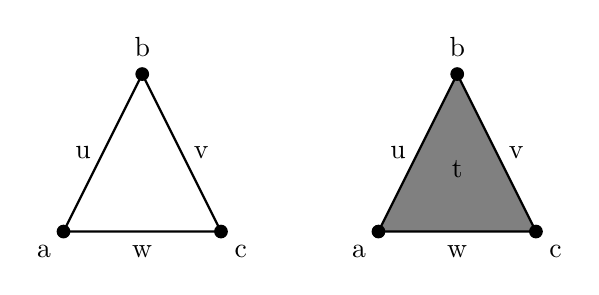
\begin{tikzpicture}
        \draw [thick] (0,0) -- (1,2) -- (2,0) -- (0,0);
        \node at (-0.25,-0.25) {a};
        \node at (1,2.35) {b};
        \node at (2.25,-0.25) {c};
        \node at (0.25,1.0) {u};
        \node at (1.75,1.0) {v};
        \node at (1,-0.25) {w};
        \draw [fill] (0,0) circle [radius=0.08];
        \draw [fill] (1,2) circle [radius=0.08];
        \draw [fill] (2,0) circle [radius=0.08];
        \draw [thick, fill=gray] (4,0) -- (5,2) -- (6,0) -- (4,0);
        \node at (3.75,-0.25) {a};
        \node at (5,2.35) {b};
        \node at (6.25,-0.25) {c};
        \node at (4.25,1.0) {u};
        \node at (5.75,1.0) {v};
        \node at (5,-0.25) {w};
        \node at (5,0.8) {t};
        \draw [fill] (4,0) circle [radius=0.08];
        \draw [fill] (5,2) circle [radius=0.08];
        \draw [fill] (6,0) circle [radius=0.08];
        \end{tikzpicture}
        \]
We begin with vertices $a$, $b$, and $c$. The vertices can be identified with a singleton set. The edges can each be identified homomorphically to $[0,1]$. We create the sides of the triangle by gluing the edges to the vertices. For example, identifying $a$ with $\{0\}$ and $b$ with $\{1\}$, we create the edge $u$. In the case of the disk, we need fill in the interior of the triangle. This is done by gluing the boundary of a disk to the edges $u$, $v$, and $w$ and letting the interior of the disk `squeeze' homeomorphically into the interior of the triangle. We have $u=[a\;\;b]$, $v=[b\;\;c]$, $w=[a\;\;c]$, and $t=[u\;\;v\;\;w]$; that is, $u$, $v$, $w$, and $t$ are convex linear combinations of vertices. We then define a sequence of maps of free $\Z$-modules on the simplices. 
	\[
	\cdots \ma{} \underbrace{0}_{\text{3-dimensional}} \ma{} \underbrace{0}_{\text{2-dimensional}} \ma{\partial_2} \underbrace{\Z u \oplus \Z v \oplus \Z w}_{\text{1-dimensional}} \ma{\partial_1} \underbrace{\Z a \oplus \Z b \oplus \Z c}_{\text{0-dimensional}} \ma{\partial_0} \underbrace{0}_{\text{(-1)-dimensional}}
	\]
We call $\partial$ the boundary map (technically, it is a collection of boundary maps $\{\delta_n\}_n$). The boundary map, $\delta_n$, creates the `edge' of a simplex of dimension $n$. In the example of the circle from above, we have $\partial_0=\partial_2=0$ and $\partial_1$ is given by
	\[
	\begin{split}
	u &\mapsto [b]-[a] \\
	v &\mapsto [c]-[b] \\
	w &\mapsto [c]-[a]
	\end{split}
	\]
Now for the disk, we have
	\[
	\cdots \ma{} \underbrace{0}_{\text{3-dimensional}} \ma{} \underbrace{\Z t}_{\text{2-dimensional}} \ma{\partial_2} \underbrace{\Z u \oplus \Z v \oplus \Z w}_{\text{1-dimensional}} \ma{\partial_1} \underbrace{\Z a \oplus \Z b \oplus \Z c}_{\text{0-dimensional}} \ma{\partial_0} \underbrace{0}_{\text{(-1)-dimensional}}
	\]
where the map $\delta_2$ is given by $t= [u\;\;v\;\;w] \mapsto u+v-w$. 


We define the $n$th homology group (that is at spot $n$) to be $H_n= \ker \partial_n/ \im \partial_{n+1}$. Since this was all motivated geometrically, there should be a geometric meaning to these homology groups. For the circle, we have $\ker \partial_1=\Z(u+v-w)$ (observe $\partial(u+v-w)=\partial(u)-\partial(v)-\partial(w)=0$) and $\im \partial_2=0$ so that $H_1(\text{circle})=\Z(u+v-w)/0 \cong \Z$. Some linear algebra (making use of the Smith Normal Form) shows that $H_0(\text{circle}) \cong \Z$. Furthermore, $\ker \partial_1$ are all the loops (cycles) in the space. It is clear that for the circle, $H_n(\text{circle})=0$ for $n \geq 2$. 


Now for the disk, we have that $\im \partial_2$ is the `boundary.' But then $H_1(\text{disk})=\ker \partial_1/\im \partial_2=\Z(u+v-w)/\Z(u+v-w)=0$; that is, the sequence is exact in that position. Some more routine linear algebra shows $H_0(\text{disk}) \cong \Z$. Finally, it is clear that $H_n(\text{disk})=0$ for $n \geq 2$. 


The geometric difference between the circle and the disk is the filled interior. Notice that in the case of the circle, $H_1(\text{circle}) \cong \Z$, a single copy of $\Z$. This represents the single 1-dimensional `hole' in the circle. Whereas for the disk, $H_1(\text{disk})=0$, representing the fact that we have `filled in' the interior. Geometrically, the rank of the $n$th homology group $H_n$, counts the number of $n$-dimensional holes. In fact, $H_0$ measure the number of connected components and $H_1$ counts the number of `traditional' holes. 


However, this notion works not just in the confines simplices but rather in the more general situation of an abelian category. We define the $n$th homology group as $H_n:=Z_n/B_n=\ker d_N/\im d_{n+1}$; that is, the $n$th homology is `cycles modulo boundaries.' Note that algebraically, $H_n$ measures how far from being exact a sequence is: $H_n=0$ if and only if the sequence is exact at $n$. Of course, as we discussed above, this has geometric meaning in many topological cases. We have now set the stage for the general theory. 



\subsection{Chain Complexes} 



\begin{dfn}[Chain Complex]
A chain complex $\dt{C}$ is a sequence of $R$-modules and maps (called differentials) $d_n$ such that the composition $d_nd_{n+1}=0$.
	\[
	\cdots \ma{} C_{n+1} \ma{d_{n+1}} C_n \ma{d_n} C_{n-1} \ma{d_{n-1}} \cdots
	\]
Whenever ambiguities will not arise, the subscripts are often omitted. The differentials then satisfy the relation $d^2=0$. 
\end{dfn}


\begin{dfn}[Cycles, Boundaries, Homology Groups]
Given a chain complex $\dt{C}$ of $R$-modules, 
	\[
	\cdots \ma{} C_{n+1} \ma{d_{n+1}} C_n \ma{d_n} C_{n-1} \ma{d_{n-1}} \cdots,
	\]
the $n$th cycle is $Z_n \defeq \ker d_n$ and the $n$th boundary is $B_n \defeq \im d_{n+1}$. Then the $n$th homology group is $H_n \defeq Z_n/B_n$. 
\end{dfn}


Note the use of subscripts instead of superscripts as the complexes are ordered in decreasing order. This will not be the case for cochain complexes and cohomology, which shall come shortly. 


\begin{ex} \hfill
	\begin{enumerate}[(i)]
	\item The following sequence is a chain complex:
		\[
		\cdots \ma{} 0 \ma{} 0 \ma{} \Z \ma{n} \Z \ma{} 0 \ma{} 0 \ma{} \cdots
		\]
	\item In a short exact sequence, $\im f =\ker g$ so that $gf=0$. But then $d^2=0$.  
	\item 
		\[
		\cdots \ma{4} \Z/8 \Z \ma{4} \Z/8\Z \ma{4} \cdots
		\]
	Notice that $d^2=16: \Z/8\Z \to \Z/8\Z$ given by $[x] \mapsto [16][x]=[0] \in \Z/8\Z$.
	\end{enumerate} \xqed 
\end{ex}


\begin{dfn}[Map of Complexes]
A morphism (map) of complexes $f: \dt{C} \to \dt{D}$ is a family of maps $f_n: C_n \to D_n$ such that the following squares commute
	\[
	\begin{tikzcd}
	\cdots \arrow{r} & C_{n+1} \arrow{r}{d_{n+1}} \arrow{d}{f_{n+1}} & C_n \arrow{r}{d_{n}} \arrow{d}{f_{n}} & C_{n-1} \arrow{r}{d_{n-1}} \arrow{d}{f_{n-1}} & \cdots \\
	\cdots \arrow{r} & D_{n+1} \arrow{r}{d_{n+1}} & D_n \arrow{r}{d_n} & D_{n-1} \arrow{r}{d_{n-1}} & \cdots 
	\end{tikzcd}
	\]
\end{dfn}


Note that the above differentials for $\dt{C}$ and $\dt{D}$ are denoted $d$, but they are not the same differential. This is an example where we will not differentiate between the two for `clarity' sake, i.e. to avoid excessive subscripts and letters. This will be done throughout these notes whenever confusion will not arise. The importance here is not whether the map is on $C_n$ or $D_n$ but that the map is a differential, moving along one of the chain complexes. 


\begin{prop}
A map of chain complexes $f: \dt{C} \to \dt{D}$ sends cycles to cycles and boundaries to boundaries. That is, $f_n(Z_n(C)) \subseteq Z_n(D)$ and $f_n(B_n) \subseteq B_n(D)$. Hence, we obtain an induced map $H_n(\dt{C}) \ma{H_n(f)} H_n(\dt{D})$. 
\end{prop}

\pf We have the following diagram:
	\[
	\begin{tikzcd}
	& Z^C_{n+1} \arrow[hook]{d} & Z^C_n \arrow[hook]{d} & Z^C_{n-1} \arrow[hook]{d} & \\
	\cdots \arrow{r} & C_{n+1} \arrow{d}{f_{n+1}} \arrow{r}{d_{n+1}} & C_n \arrow{d}{f_n} \arrow{r}{d_n} & C_{n-1} \arrow{d}{f_{n-1}} \arrow{r}{d_{n-1}} & \cdots \\
	\cdots \arrow{r} & D_{n+1} \arrow{r}{\ov{d}_{n+1}} & D_n \arrow{r}{\ov{d}_n} & D_{n-1} \arrow{r}{\ov{d}_{n-1}} & \cdots  \\
	& Z^D_{n+1} \arrow[hook]{u} & Z^D_n \arrow[hook]{u} & Z^D_{n-1} \arrow[hook]{u} & 
	\end{tikzcd}
	\]
where $Z_n^C$ and $B_n^C$ are the $n$th cycles and boundaries of $\dt{C}$, respectively, and $Z_n^B$ and $B_n^D$ are the $n$th cycles and boundaries of $\dt{D}$, respectively. Suppose that $x \in Z^C_n$, i.e. $d_n(x)=0$. Then $f_{n-1}(d_n(x))=0$. By commutativity, $\ov{d}(f_n(x))=0$. But then $f_n(x) \in \ker \ov{d}_n=Z^D_n$. Hence, $f_n(Z_N^C) \subseteq Z_n^D$. So $f$ sends cycles to cycles. Now let $y \in B^C_n$. Then there is a $c \in C_{n+1}$ such that $d_{n+1}(c)=y$. By commutativity, $\ov{d}_{n+1}(f_{n+1}(c))=f_n(d_{n+1}(c))=f_n(y)$. But then $f_n(y)= \ov{d}_{n+1}(b)$, where $b:= f_{n+1}(c)$. Therefore, $f_n(y) \in Z_n^D$. So $f$ sends boundaries to boundaries. Therefore, $f$ induces a map $H_n(f): H_n(C) \to H_n(D)$ given by $\ov{c} \mapsto f(\ov{c})$. \qed \\


\begin{dfn}[Kernel/Cokernel of a Map of Complexes]
For a map of complexes $f: \dt{C} \to \dt{D}$, define $\ker f$ to be the complex
	\[
	\cdots \ma{} \ker f_n \ma{d_n^C |_{\ker}} \ker f_{n-1} \ma{} \cdots
	\]
and $\coker f$ to be the complex
	\[
	\cdots \ma{} \coker f_n \ma{d_n^C |_{\coker}} \coker f_{n-1} \ma{} \cdots
	\]
\end{dfn}


\begin{dfn}[Subcomplex]
If $\dt{C}$ is a complex, we say that $\dt{B}$ is a subcomplex of $\dt{C}$ if $B_n \subset C_n$ for all $n$ and $d_n^B=d_n^C |_{B_n}$.
\end{dfn}


\begin{dfn}[Quotient Complex]
If $\dt{B}$ is a subcomplex of $\dt{C}$, the quotient complex, written $C/B$ or $\dt{C}/\dt{B}$, is the complex
	\[
	\cdots \ma{\ov{d}} C_{n+1}/B_{n+1} \ma{\ov{d}} C_n/B_n \ma{\ov{d}} \cdots
	\] 
with differentials given by $\ov{d}(\ov{x})=\ov{d(x)}$. Furthermore, $B \to C \to C/B$ are chain maps, as maps of complexes. 
\end{dfn}


\begin{dfn}[Kernel, Cokernel, and Image of Complex Maps]
Given a chain map $f: \dt{C} \to \dt{D}$, then the individual modules $\ker f_n$, $\coker f_n$, and $\im f_n$ and maps induced by the differentials of $C$ or $D$ form complexes called $\ker f \subseteq C$, $\coker f=D/\im f$, $\im f \subseteq D$. 
\end{dfn}


In fact, these really are the categorical $\ker$, $\coker$, and $\im$ of $f$ in the category \textbf{Ch(R-mod)}, the category of chain complexes of $R$-modules. In this category, the objects are chain complexes of $R$-modules and the morphisms are chain maps. Observe that \textbf{Ch(R-mod)} is abelian. Furthermore, if \textbf{A} is an abelian category, then \textbf{Ch(A-mod)} is abelian. A sequence of complexes $\dt{0} \to \dt{A} \to \dt{B} \to \dt{C} \to \dt{0}$ is an exact sequence of chain complexes if and only if each one (in each degree) is exact; that is, if $0 \to A_n \to B_n \to C_n \to 0$ is exact. Having all the language of complexes in place, we define cochain complxes. 


\begin{dfn}[Cochain Complex]
A cochain complex $\udt{C}$ is a sequence of $R$-modules and maps $\{d_n\}$ with $d^2=0$.
	\[
	\cdots \ma{} C^{n-1} \ma{d^{n-1}} C^n \ma{d^n} C^{n+1} \ma{d^{n+1}} \cdots
	\]
\end{dfn}


Note that a cochain complex is just a chain complex with increasing indices. We can convert one to the other by reindexing $C_{-n}:= C^n$ for all $n \in \Z$. 


\begin{dfn}[Cocycles, Coboundary, Cohomology]
Given a cochain complex $\udt{C}$, we define the $n$th cocycle as $Z^n=\ker d^n$, the $n$th coboundary  as $B^n=\im d^{n-1}$, and the $n$th cohomology group to be $H^n(C^n)=Z^n/B^n$. 
\end{dfn}


We have defined the notion of homology and maps between complexes. Now we define a special class of morphisms between complexes. 


\begin{dfn}[Quasi-Isomorphism]
A chain map $f: \dt{C} \rightarrow \dt{D}$ is called a quasi-isomorphism if it induces an isomorphism on homology, $H_n(f): H_n(\dt{C}) \ma{\sim} H_n(\dt{D})$, for all $n$. A quasi-isomorphism is also called a quism, quiz, or q-iso. 
\end{dfn}


\begin{rem} \hfill
	\begin{enumerate}[(i)]
	\item It is clear that $\dt{C}$ is exact if and only if $H_n(C)=0$ for all $n$. Furthermore, $\dt{0} \rightarrow \dt{C}$ is a quasi-isomorphism if and only if $\dt{C} \rightarrow \dt{0}$ is a quasi-isomorphism. 
	\item Not every complex is quasi-isomorphic to its homology as there need not necessarily exist a map between them. Therefore, it is possible to have two complexes $C,D$ with the same homology groups but that are not quasi-isomorphic, see Example~\ref{ex:quism}.
	\end{enumerate}
\end{rem}


\begin{ex}
Let $\dt{C}$ be the following complex
	\[
	\cdots \ma{4} \Z/12\Z \ma{3} \Z/12\Z \ma{4} \Z/12\Z \ma{3} \Z/12\Z \rightarrow 0
	\]
We have $H_0(C)=\ker d_0/\im d_1=(\Z/12\Z)/(3\Z/12\Z) \cong \Z/3\Z$---the cokernel of $d_1$. Furthermore, $H_1(C)=(4\Z/12\Z)/(4\Z/12\Z) \cong 0$, and $H_2(C)=(3\Z/12\Z)/(3\Z/12\Z) \cong 0$. Therefore, we have
	\[
	H_n(C) \cong
	\begin{cases}
	\Z/3\Z, & \text{ if }n=0 \\
	0, & \text{ otherwise}
	\end{cases}
	\]
So this sequence is exact at all $n$ with the exception of $n=0$. Consider the following diagram of chain complexes:
	\[
	\begin{tikzcd}
	\cdots \arrow{r} & \Z/12\Z \arrow{d} \arrow{r}{4} & \Z/12\Z \arrow{d} \arrow{r}{3} & \Z/12\Z \arrow{r} \arrow{d}{\pi} & 0 \\
	\cdots \arrow{r} & \arrow{r} 0 \arrow{r} & 0 \arrow{r} & \Z/3\Z \arrow{r} & 0
	\end{tikzcd}
	\]
It is clear that the squares commute (only the last square is a concern but $\pi \circ 3=0$ in $\Z/3\Z$). The above computations so that the following is a chain map of complexes. The bottom row clearly has homology groups $H_n=0$ for $n \geq 1$ and $H_0= \ker d_0/\im d_1= (\Z/3\Z)/0= \Z/3\Z$. Therefore, the above map of chain complexes is a quasi-isomorphism. \xqed
\end{ex}


\begin{ex} \label{ex:quism}
Take the following two complexes
	\[
	\begin{split}
	C:\;\; & 0 \longrightarrow \Z/4\Z \ma{2} \Z/4\Z \longrightarrow 0 \\
	D:\;\; & 0 \longrightarrow \Z/2\Z \ma{0} \Z/2\Z \longrightarrow 0
	\end{split}
	\]
These complexes have isomorphic homology groups but are not quasi-isomorphic: the induced maps on homology are the zero maps but these complexes both have nonzero homology groups. \xqed
\end{ex}



\subsection{Long Exact Sequences}
















































To understand how homologies behave, we now need to develop the most useful tool for any good homology theory - long exact sequences. 

\begin{thm}
Let $\dt{0} \longrightarrow \dt{A} \ma{f} \dt{B} \ma{g} \dt{C} \longrightarrow 0$ be a short exact sequence of chain complexes. Then for all $n$, there are natural maps $\delta: H_n(C) \rightarrow H_{n-1}(A)$, called connecting homomorphisms, such that the sequence
\[
\cdots \rightarrow H_{n+1}(A) \longrightarrow H_{n+1}(B) \longrightarrow H_{n+1}(C) \ma{\delta_{n+1}} H_n(A) \ma{H_n(f)} H_n(B) \ma{H_n(g)} H_n(C) \ma{\delta_n} H_{n-1}(A) \longrightarrow \cdots
\] 
is exact. Similarly, if instead we have a short exact sequence of cochain complexes, then for all $n$ there are natural maps $\delta: H^n(C) \rightarrow H^{n+1}(A)$ such that the sequence
\[
\cdots \rightarrow H_{n+1}(A) \longrightarrow H_{n+1}(B) \longrightarrow H_{n+1}(C) \ma{\delta_{n+1}} H_n(A) \ma{H_n(f)} H_n(B) \ma{H_n(g)} H_n(C) \ma{\delta_n} H_{n-1}(A) \longrightarrow \cdots
\] 
is exact. 
\end{thm}

Proof: This is just a simple application of the Snake Lemma. Given a short exact sequence of complexes $0 \ma{} \dt{A} \ma{} \dt{B} \ma{} \dt{C} \ma{} 0$, apply the Snake Lemma to 
\[
\begin{tikzcd}
0 \arrow{r} & A_n \arrow{r} \arrow{d}{d_n^A} & B_n \arrow{r} \arrow{d}{d_n^B} & C_n \arrow{r} \arrow{d}{d_n^C} & 0 \\
0 \arrow{r} & A_{n-1} \arrow{r} & B_{n-1} \arrow{r} & C_{n-1} \arrow{r} & 0 
\end{tikzcd}
\]
in order to get for each $n$ an exact sequence
\[
0 \ma{} Z_{n}^A \ma{} Z_{n}^B \ma{} Z_{n}^C \ma{\delta} A_{n-1}/\im d_n^A \ma{} B_{n-1}/\im d_n^B \ma{} C_{n-1}/\im d_n^C \ma{} 0 
\]
We rearrange to a commutative diagram with exact rows 
\[
\begin{tikzcd}
\phantom{x} & A_n/\im d_n \arrow{r} \arrow{d} B_n/\im d \arrow{r} \arrow{d} & C_n/\im d \arrow{r} \arrow{d} & 0 \\
0 \arrow{r} & Z_{n-1}^A \arrow{r} & Z_{n-1}^B \arrow{r} & Z_{n-1}^C & 
\end{tikzcd}
\]
Applying the Snake Lemma we get an exact sequence
\[
H_n(A) \ma{} H_n(B) \ma{} H_n(C) \ma{\delta} H_{n-1}(A) \ma{} H_{n-1}(B) \ma{} H_{n-1}(C)
\]
\qed \\

Note that we often write long exact sequences of homology groups as follows: given an exact sequence of complexes $0 \ma{} \dt{A} \ma{} \dt{B} \ma{} \dt{C} \ma{} 0$, we write the exact sequence of homology groups as
\[
\begin{tikzcd}
H_*(A) \arrow{rr} & & H_*(B) \arrow{dl} \\
& H_*(C) \arrow{ul}{\delta} & 
\end{tikzcd}
\]

\begin{prop}[Naturality of Long Exact Sequence]
The map $\delta$ is natural; that is, given a commutative diagram of complexes
\[
\begin{tikzcd}
0 \arrow{r} & \dt{A} \arrow{r} \arrow{d}{\alpha} & \dt{B} \arrow{r} \arrow{d}{\beta} & \dt{C} \arrow{r} \arrow{d}{\gamma} & 0 \\
0 \arrow{r} & \dt{A'} \arrow{r} & \dt{B'} \arrow{r} & \dt{C'} \arrow{r} & 0 
\end{tikzcd}
\]
the following diagram commutes
\[
\begin{tikzcd}
\cdots \arrow{r} & H_n(B) \arrow{r} \arrow{d}_{H_n(\beta)} & H_n(C) \arrow{r}{\delta} \arrow{d}{H_n(\gamma)} & H_{n-1}(A) \arrow{r} \arrow{d}{H_n(\alpha)} & \cdots \\
\cdots \arrow{r} & H_n(B) \arrow{r} & H_n(C) \arrow{r}{\delta}  & H_{n-1}(A) \arrow{r} & \cdots
\end{tikzcd}
\]
\end{prop}

Proof: The squares with only $H_n(-)$ clearly commute as $H_n$ is a functor: $H_n(fg)=H_n(f) H_n(g)$ for all composable $f,g$, as is easy to check. For the squares with the $\delta$'s, note that $\delta$ is constructed in the same way as they are in the Snake Lemma. If one lifts $\ov{c} \in H_n(C)$ to a $b \in B_n$ and $d(b)$ is the image of $a \in A_{n-1}$,
\[
\begin{tikzcd}
0 \arrow{r} & A_n \arrow{d} \arrow{r} & B_n \arrow{r} \arrow{d} & C_n \arrow{r} \arrow{d} & 0 \\
& A_{n-1} \arrow{r} & B_{n-1} \arrow{r} & C_{n-1} & 
\end{tikzcd}
\]
then $\beta(b)$ lifts $\gamma(\ov{c})=\ov{\gamma(c)}$. As $\beta$ is a chain map, we know $d(\beta(b))=\beta(d(b))$ is the image of $\alpha(a)$. So $\delta(\ov{\gamma}(c))=\ov{\alpha(a)}$. So the square commutes
\[
\delta(\ov{\gamma}(\ov{c}))= \ov{\alpha}(\ov{a})=\ov{\alpha}(\delta(\ov{c}))
\]
\qed \\

\subsection{Homotopy} 

\begin{dfn}
A complex is split exact if it is exact and for all $n$
\[
0 \ma{} Z_n \ma{\subseteq} C_n \ma{d} B_{n-1} \ma{} 0
\]
is split exact. 
\end{dfn}

Note that you actually get $C_n=Z_n \oplus s(B_{n-1})$ and $C$ is the following complex $X_n=s(B_{n-1})$
\[
\begin{tikzcd}
Z_{n+1} & Z_n & Z_{n-1} & \\
\oplus \arrow{r} & \oplus \arrow{r}  & \oplus \arrow{r} & \cdots \\
X_{n+1} \arrow{uur}{\sim} & X_n \arrow{uur}{\sim} & 
\end{tikzcd}
\]
where $d(s(B_{n-1}))=1_{B_{n-1}}$. Furthermore, any exact complex $C$ over a field (or semisimple ring) is split exact. However, less ``drastic" is the notion of homotopy. 

\begin{dfn}[Nulltomotopy]
A chain map $f: \dt{C} \to \dt{D}$ is nullhomotopic $f \simeq 0$ if there are maps $s_n: C_n \to D_{n+1}$ such that $f=ds'+sd$. The map $s$ is called a (null)homotopy. 
\[
\begin{tikzcd}
\cdots \arrow{r} & C_{n+1} \arrow{r}{d} \arrow{d}{f} \arrow{dl}{s} & C_n \arrow{r}{d} \arrow{d} \arrow{dl}{s} & C_{n-1} \arrow{r} \arrow{d}{f} \arrow{dl}{s} & \cdots \arrow{dl}{s} \\
\cdots \arrow{r} & D_{n+1} \arrow{r}{d'} & D_n \arrow{r}{d'} & D_{n-1} \arrow{r}{d'} & \cdots 
\end{tikzcd}
\]
Two chain maps $f,g: \dt{C} \to \dt{D}$ are homotopic $f\simeq g$ if $f-g$ is nullhomotopic, i.e. $f-g \simeq 0$. Finally, $f: \dt{C} \to \dt{D}$ is a homotopy equivalence if it has an inverse up to homotopy; that is, there is $g: D \to C$ such that $fg \simeq 1_D$ and $gf \simeq 1_C$. 
\end{dfn}

\begin{prop}
If $f\simeq 0$ then $H(f)=0$. Therefore, $f \simeq g$ then $H(f)=H(g)$ as maps.
\end{prop}

Proof: Given a chain map $f: \dt{C} \to \dt{D}$. If $f \simeq 0$, then there is $s: f=sd+d's$.
\[
\begin{tikzcd}
\phantom{x} & C_n \arrow{r}{d} \arrow{dl} \arrow{d}{f} & C_{n-1} \arrow{dl}{s} \\
D_{n+1} \arrow{r}{d'} & D_n & 
\end{tikzcd}
\]
If $\ov{x} \in H_n(C)= Z_n/B_n$, then 
\[
\begin{split}
f(x)&=(sd+d's)(x) \\
&=(sd)(x)+(d's)(x) \\
&=s(d(x))+0 \\
&=s(0) + 0 \\
&= 0 + 0 \\
&= 0 
\end{split}
\]
Note that $d(s(x)) \in B_n$ so $(d's)(x)$, which is 0 in $H_n(D)$. Then $f \simeq g$ so that $f-g \simeq 0$ by the above. So $H_n(f-g)=0$ so that $H_n(f)=H_n(g)$. \qed \\

\begin{prop}
$C$ is split exact if and only if $1_C \simeq 0$. 
\end{prop}

\begin{ex}
Take $R=\Z[x,y]/(xy)$. 
\[
\cdots \ma{x} R \ma{x} R \ma{x} R \ma{x} R \ma{} 0 
\] 
and multiplication by $x$ on $\dt{C}$. We claim that $x \simeq 0$. 
\[
\begin{tikzcd}
\cdots \arrow{r} & R \arrow{r}{x} \arrow{d}{x} \arrow{dl}{s} & R \arrow{r}{x} \arrow{d}{x} \arrow{dl}{s} & R \arrow{r} \arrow{d}{x} \arrow{dl}{s} & \cdots \arrow{dl}{s} \\
\cdots \arrow{r} & R \arrow{r}{x} & R \arrow{r}{x} & R \arrow{r}{x} & \cdots 
\end{tikzcd}
\]
Create $s$ by taking the zero map or the identity in the appropriate places. This also shows that homotopies are not necessarily unique as we could have chosen $s=x$ everywhere. 
\end{ex}

\subsection{Bicomplexes and Tot}

\begin{dfn}[Bicomplex]
A double complex or bicomplex is a diagram of $R$-modules and maps
\[
\begin{tikzcd}
\phantom{x} & \vdots \arrow{d} & \vdots \arrow{d} & \\
\cdots & C_{p-1,q} \arrow{l} \arrow{d}{d'} & C_{p,q} \arrow{l}{d} \arrow{d}{d'} & \cdots \arrow{l} \\
\cdots & C_{p-1,q-1} \arrow{l} \arrow{d}{d'} & C_{p,q-1} \arrow{l}{d} \arrow{d}{d'} & \cdots \arrow{l} \\
& \vdots & \vdots & 
\end{tikzcd}
\]
where $d^2=0$, $d'^2=0$, and that the diagram commutes, i.e. $dd'=d'd$. 
\end{dfn}

\begin{enumerate}[1.]
\item We can think that a bicomplex as a complex of complexes (vertical or horizontal). 
\item The index is the position in $(x,y)$ in Cartesian coordinates. The arrows are usually drawn to all flow towards the origin or all to flow away from the origin. 
\item Some authors have all squares in the diagram anticommute: $dd'= - d'd$. 
\item $\ddt{C}$ is bounded if along each diagonal $p+q=n$ (fixed) there are only finitely many nonzero modules. For example, a first quadrant bicomplex is bounded. 
\end{enumerate}

\begin{dfn}[Total Complex]
Given a bicomplex $C$, form the total complex $\tot(C)$ as
\[
\begin{split}
\left( \tot \bigoplus C \right)_n &\defeq \bigoplus_{p+q=n} C_{p,q} \\
\left( \tot \prod C \right)_n \defeq \prod_{p+q=n} C_{p,q}
\end{split}
\]
with differentials $d^{\tot} \defeq d+(-1)^pd'$. 
\end{dfn}

\begin{rem}
We place the minus sign on odd columns to make the diagram anticommute. If $\ddt{C}$ is bounded, then $\tot \oplus= \tot \prod$. One can check that this diagram does indeed anticommute and $(d^{\tot})^2=0$ so that this indeed a complex. 
\end{rem}

\begin{ex}
Given two complexes
\[
\dt{P}: \cdots \ma{} P_1 \ma{} P_0 \ma{} 0 
\]
\[
\dt{Q}: \cdots \ma{} Q_1 \ma{} Q_0 \ma{} 0
\]
Then the tensor product $\dt{P} \otimes_R \dt{Q}$ is a bicomplex
\[
\begin{tikzcd}
\vdots \arrow{d} & \vdots \arrow{d} & & \\
P_0 \otimes_R Q_2 \arrow{d} & P_1 \otimes_R Q_2 \arrow{d} \arrow{l} & & \\
P_0 \otimes_R Q_1 \arrow{d} & P_1 \otimes_R Q_1 \arrow{d} \arrow{l} & \ddots \arrow{l} \arrow{d} & \\
P_0 \otimes_R Q_0  & P_1 \otimes_R Q_0 \arrow{l}{d \otimes 1} & P_2 \otimes_R Q_0  \arrow{l}{d \otimes 1} & P_3 \otimes_R Q_0 \arrow{l}{d \otimes 1} 
\end{tikzcd}
\]
or its Tot
\[
(\dt{P} \otimes_R \dt{Q})_n = \bigoplus_{p+q=n} P_p \otimes_R Q_q
\]
Similarly, we can define a bicomplex from $\Hom_R(\dt{P},\dt{Q})$.
\end{ex}

Furthermore, if $0 \ma{} \ddt{A} \ma{} \ddt{B} \ma{} \ddt{C} \ma{} 0$ is an exact sequence of bicomplexes and are bounded, then there is a short exact sequence. To see this, note that the direct sum of finitely many short exact sequences is exact and that if $A \to B$ is a map of bicomplexes then the map $\tot(A) \to \tot(B)$ is a map. 

\subsection{Mapping Cone \& Mapping Cylinder}

\begin{dfn}[Mapping Cone]
Let $f: \dt{B} \to \dt{C}$ be a chain map, then the mapping cone of $f$ is $C(f) \defeq \tot(C \stackrel{\longleftarrow}{f})$
\[
\begin{tikzcd}
C_3 \arrow{d}{d} & B_3 \arrow{l} \arrow{d}{-d'} \\
C_2 \arrow{d}{d} & B_2 \arrow{l} \arrow{d}{-d'} \\
C_1 \arrow{d}{d} & B_1 \arrow{l} \arrow{d}{-d'} \\
C_0 & B_0 \arrow{l}{f}
\end{tikzcd}
\]
$\left(C(f)\right)_n=C_n \oplus B_{n-1}$
\[
\begin{tikzcd}
C_n \arrow{r}{d} & C_{n-1} \\
\oplus & \oplus \\
B_{n-1} \arrow{uur}{f} \arrow{r}{-d} & B_{n-2}
\end{tikzcd}
\]
with differential $\begin{bmatrix} d & f \\ 0 & -d \end{bmatrix}$. 
\end{dfn}

\begin{prop}
\begin{enumerate}[1.]
\item There is a short exact sequence of complexes
\[
0 \ma{} C \ma{i_1} C(f) \ma{\pi_2} B[-1] \ma{} 0 
\]
where $B[-1]$ is the complex $B$ shifted one unit to the left, i.e. $(B[-1])_n=B_{n-1}$. 
\item There is an associated long exact sequence of homology
\[
\cdots \ma{\delta} H_n(C) \ma{} H_n(C(f)) \ma{} H_n(B[-1]) \ma{\delta} H_{n-1}(C) \ma{} H_{n-1}(C(f)) \ma{} \cdots
\]
with connecting map $\delta=H_n(f)$. 
\item The map $f$ is a quasi-isomorphism if and only if $H_n(C(f))=0$. 
\end{enumerate}
\end{prop}

\begin{dfn}[Mapping Cylinder]
Let $f: \dt{B} \to \dt{C}$ be a chain map. The mapping cylinder of $f$ is $\cyl(f) \defeq C(C(f)[1] \ma{\pi_2} B)$. One could think of this as ``Tot" of $(C \stackrel{f}{\longleftarrow} B \ma{} B)$. However, the arrows go the other way but this is a tricomplex. Also, $(\cyl(f))_n\defeq C_n \oplus B_{n-1} \oplus B_n$ with the obvious differentials. 
\end{dfn}

Essentially, we have subtracted off the complex $B$ from the cone up to homology. To verify this instinct, we prove the following lemma.

\begin{lem}
There is an exact sequence
\[
0 \ma{} C \ma{i} \cyl(f) \ma{} C(1_B)[-1] \ma{} 0 
\]
But $C(1_B)$ is always split exact. Hence by the long exact sequence, $H(i)$ is an isomorphism so that $i$ is a quasi-isomorphism. In fact, $i$ is a homotopy equivalence. 
\end{lem}

Proof: Look at $\cyl(f) \ma{j} C$ given by $(C,b,b') \mapsto c+f(b)$. One need check the following details:
\begin{itemize}
\item This is a chain map
\item The composition $ji=1_C$
\item $c \mapsto (c,0,0) \mapsto c+f(0)=c$
\item $ij \simeq 1_{\cyl(f)}$
\end{itemize}

\begin{lem}
There is a commutative diagram
\[
\begin{tikzcd}
 \phantom{x} & B \arrow{r}{f} \arrow{d}{\cong} & C \arrow[xshift=1ex]{d}{j} \arrow{r}{i} & C(f) \arrow{d}{\cong} & \\
 0 \arrow{r} & B \arrow{r}{i_3} & \cyl(f) \arrow[xshift=-1ex]{u}{i} \arrow{r} & C(f) \arrow{r} & 0 
\end{tikzcd}
\]
\end{lem}

\begin{rem}
The above lemma is useful for triangulated and derived categories.
\end{rem}


\newpage